\ifx\boi\undefined\ifx\problemname\undefined
\providecommand\sampleinputname{}
\providecommand\sampleoutputname{}
\documentclass[english]{templates/boi}
\problemlanguage{.en}
\fi
\newcommand{\boi}{Baltic Olympiad in Informatics}
\newcommand{\practicesession}{Practice Session}
\newcommand{\contestdates}{April 27 - May 1, 2018}
\newcommand{\dayone}{Day 1}
\newcommand{\daytwo}{Day 2}
\newcommand{\licensingtext}{This problem is licensed under CC BY-SA 4.0.}
\newcommand{\problem}{Problem}
\newcommand{\inputsection}{Input}
\newcommand{\outputsection}{Output}
\newcommand{\interactivity}{Interactivity}
\newcommand{\grading}{Grading}
\newcommand{\scoring}{Scoring}
\newcommand{\constraints}{Constraints}
\renewcommand{\sampleinputname}{Sample Input}
\renewcommand{\sampleoutputname}{Sample Output}
\newcommand{\sampleexplanation}[1]{Explanation of Sample #1}
\newcommand{\sampleexplanations}{Explanation of Samples}
\newcommand{\timelimit}{Time Limit}
\newcommand{\memorylimit}{Memory Limit}
\newcommand{\seconds}{s}
\newcommand{\megabytes}{MB}
\newcommand{\group}{Group}
\newcommand{\points}{Points}
\newcommand{\limitsname}{Limits}
\newcommand{\additionalconstraints}{Additional Constraints}
\newcommand{\testgroups}{
Your solution will be tested on a set of test groups, each worth a number of points.
Each test group contains a set of test cases.
To get the points for a test group you need to solve all test cases in the test group.
Your final score will be the maximum score of a single submission.
}
\fi
\def\version{jury-1}
\problemname{Armastuse hulknurk}
Nagu me kõik teame, on seebiooperite tegelased omavahel tõsiselt keerulistes suhetes. Ühes seebiooperis on $N$ 
tegelast, kellest igaüks armastab täpselt üht isikut. On ka võimalik, et tegelane armastab (alguses) ainult iseennast. Ütleme, et kaks tegelast on paarisuhtes, kui esimene armastab teist ja teine esimest.

Vahel tekib eriti keeruline suhe, mida nimetatakse ``armastuse hulknurgaks''.
Ütleme, et 3 või enam inimest on ``armastuse hulknurgas'', kui esimene armastab teist, teine kolmandat jne,
kuni viimane isik armastab esimest.

Vaatajaküsitlused näitavad, et televaatajad on sellisest draamast väsinud nig eelistaks midagi romantilisemat.
Meil on võimalik muuta, keda inimene armastab, tulistades teda armunoolega. Eesmärgiks on, et kõik isikud oleksid paarisuhetes.

Mis on minimaalne arv armunooli, mis selleks tuleb kulutada?

\section*{\inputsection}
Esimesel real on täisarv $N$, mis tähistab seebiooperi tegelaste arvu.
Järgmistel $N$ real on igaühel kaks tühikuga eraldatud nime $s$ ja $t$, mis tähendavad, et tegelane $s$ 
armastab alguses tegelast $t$. Nimed on ülimalt $10$ tähe pikkused ja koosnevad ladina tähestiku väiketähtedest.

\section*{\outputsection}
Väljundisse kirjutada üks täisarv -- minimaalne armunoolte arv, mis kindlustaks, et kõik tegelased on suhtes.
Kui see ei ole võimalik, väljastada \texttt{-1}.

\section*{\constraints}
\testgroups

\noindent
\begin{tabular}{| l | l | l | l |}
\hline
\group & \points & \limitsname & \additionalconstraints \\ \hline
1     & 21     & $2 \le N \le 20$ & \\ \hline
2     & 25     & $2 \le N \le 100\,000$ & Iga isiku puhul leidub keegi, kes teda armastab (võimalik, et ta ise). \\ \hline
3     & 29     & $2 \le N \le 100\,000$ & Alguses pole ühtki paarisuhet ega ``armastuse hulknurka''. \\ \hline
4     & 25     & $2 \le N \le 100\,000$ & \\ \hline
\end{tabular}

\section*{\sampleexplanations}

\begin{center}
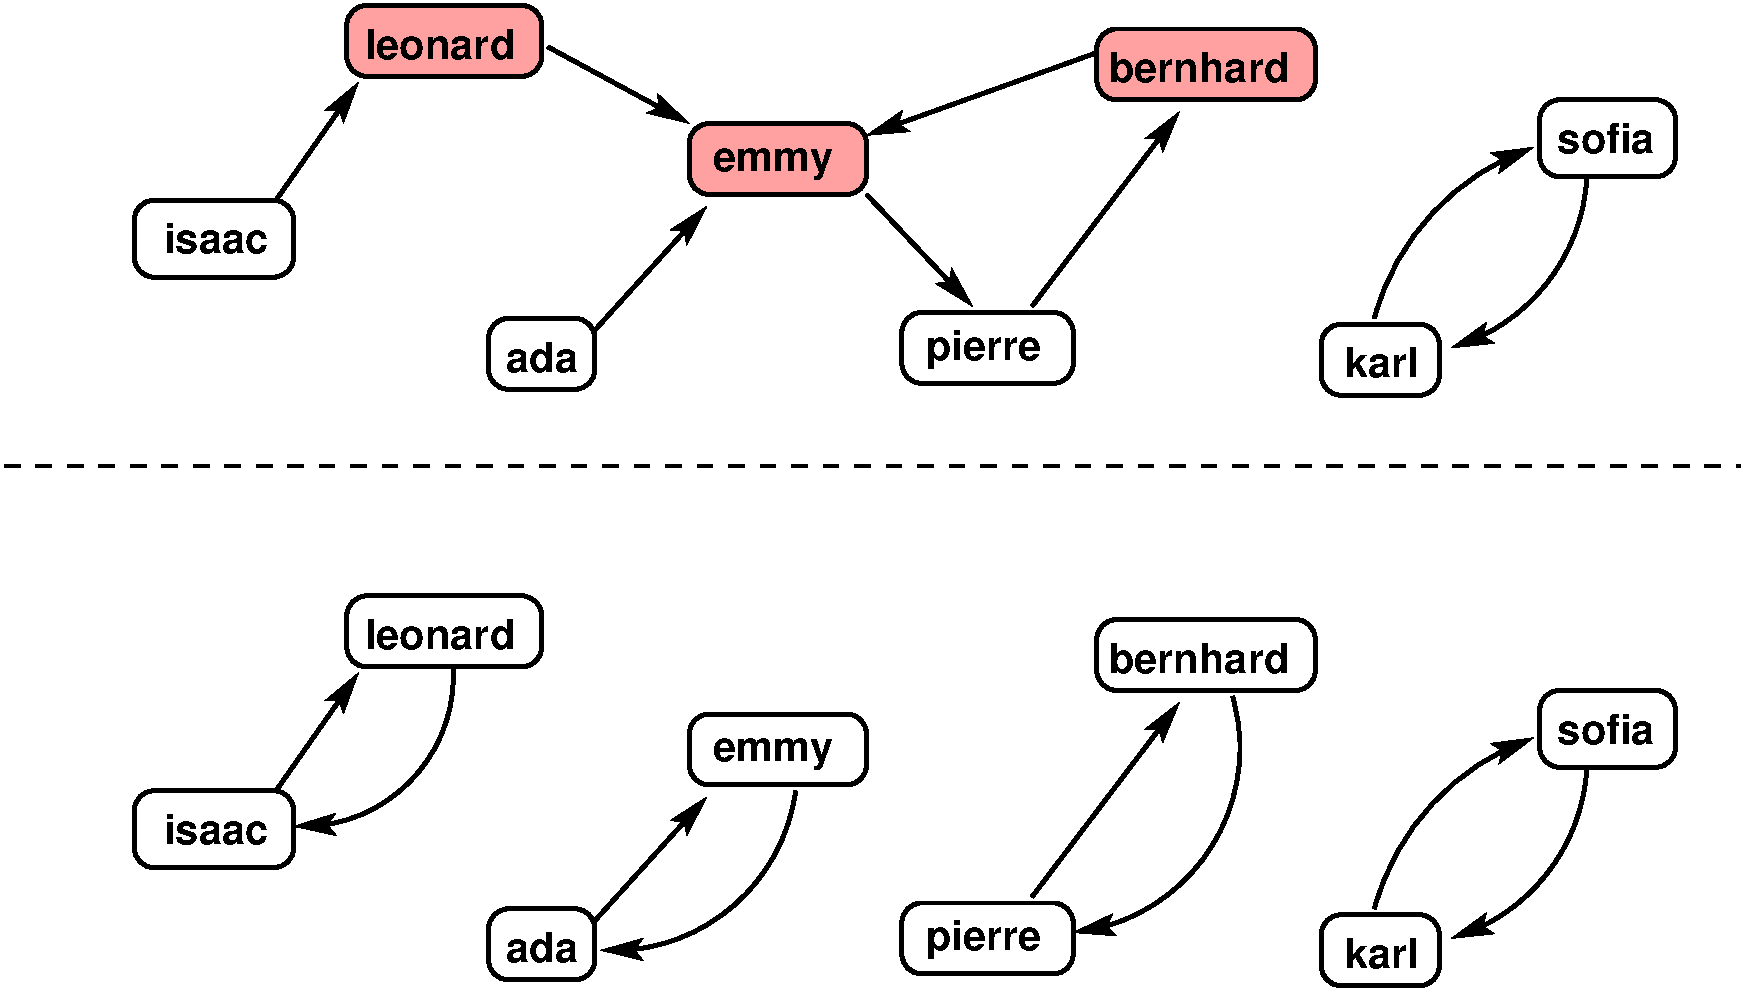
\includegraphics[width=0.5\textwidth]{polygonfig.pdf}
\end{center}

Esimene näide on toodud joonisel. Ülemine osa illustreerib algset olukorda, kus nool, mis näitab isikult $s$ isikule $t$, 
tähendab, et isik $s$ armastab alguses isikut $t$, ning roosa värv tähistab kolme isikut, keda tuleb optimaalse olukorra 
saavutamiseks tulistada. Alumine osa näitab lõppseisu.
%Esimeses näites on ainsaks lahendiks: tulistada
%isikuid \texttt{b}, \texttt{d} ja \texttt{f} armunooltega, mis tähendab, et nad hakkavad armastama vastavalt isikkuid \texttt{h}, \texttt{c} ja \texttt{e}.

Teises näites (mis rahuldab alamülesande 3 tingimusi) on mitu võimalikku lahendust.
Üks võimalus on tulistada iskuid \texttt{a}, \texttt{b} and \texttt{d}, nii et nad hakkavad armastama isikuid \texttt{b}, \texttt{a} ja \texttt{c}.

Kolmandas näites on meil armastuse kolmnurk ja ükskõik, kuidas nooli lasta, jääb keegi alati välja.
